\section{Exploratory Data Analysis}
We analyze the best seller and worst seller products across the various stores and provide our analysis. 
\subsection{Product analysis based on inventory}
For all stores except 18, 117, and 332, we can visually determine which stores have the highest average received quantities over the span of one year. For products which appear to have some of the highest received quantities such as the everything bagel, butter croissant, and danish classic cheese, this may indicate a high demand for these products as the stores need to stock up or a precursor to how much waste is generated by not selling enough of said product. Likewise, we can apply the same logic towards the lower end of products such as the caprese sandwich and pretzel egg sandwich, where perhaps there is not enough demand for these items, resulting in lower received quantities. 

\begin{figure}[ht]
    \centering
    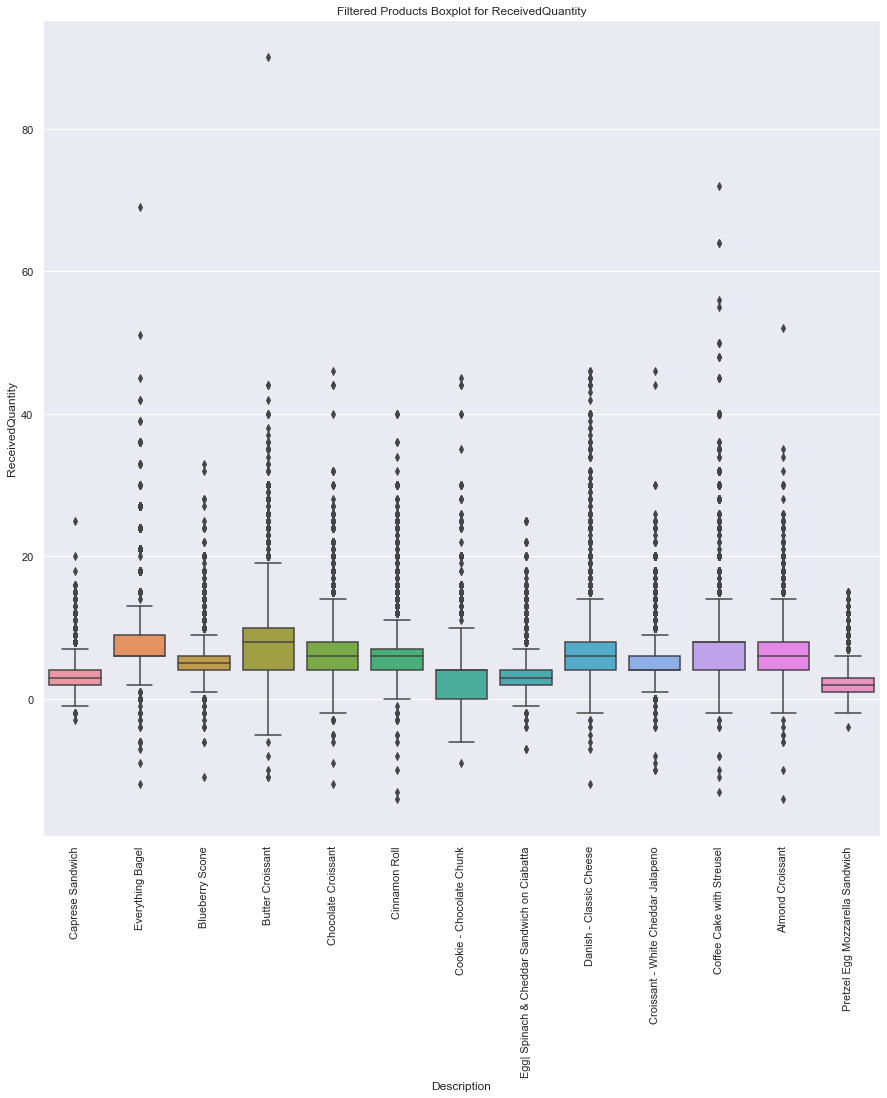
\includegraphics[width = 0.7\linewidth]{figures/figure1.png}
    \caption{Analysis for highest average received quantities }
\end{figure}

The last detail worth mentioning about this graph is that every product present in these stores accordingly reaches at least one negative value in their received quantity. What this indicates to us is perhaps products that may never made it to stores during transit or lost in some way. However, it is worth mentioning that by manually searching through said data, these data points are few and far in between, so this may not be an issue to be concerned with overall, but still possibly worth investigating.

\\

Figure 2 graph may be the most impactful in understanding the rank order of how consistently products sell overall compared to one another, and may indicate preferences among customers. For example, the butter croissant, everything bagel, and coffee cake appear to be the most consistent products in this list, with decently well situated averages as shown in the box plot. This may be a suggestion to look at these products more closely to try and understand how to further increase sales due to their sell out quantities. 
\begin{figure}[ht]
    \centering
    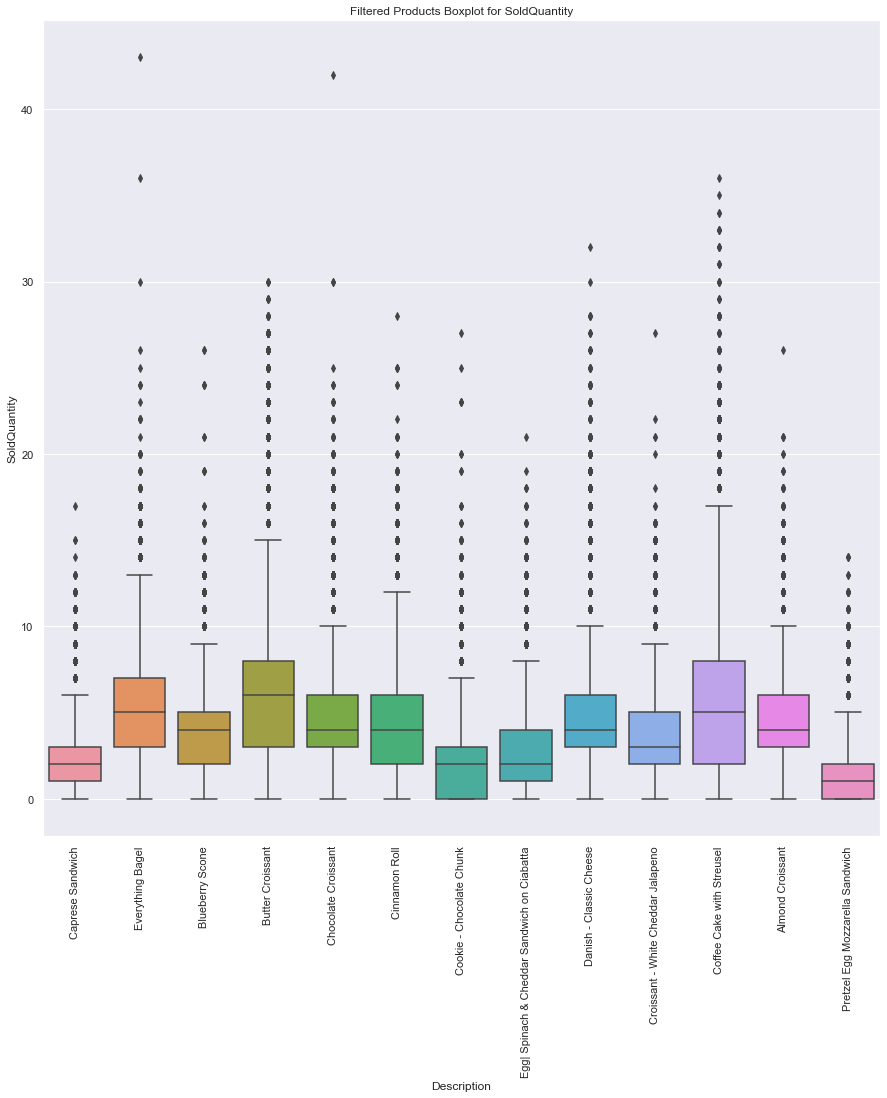
\includegraphics[width = 0.7\linewidth]{figures/figure2.png}
    \caption{Analysis for highest average received quantities }
\end{figure}
Our last note on this is to see how the received quantities of all products compare to their sold quantities, as we would preferably want to see a close relation between the two. Previously we have already mentioned that butter croissants and everything bagel have high received quantities, possibly indicating either a high demand or a precursor to waste. Here we can more confidently say that since the sold quantities of said products appear to be fairly consistent, we may believe that those products are not being wasted or tossed.

\\
Figure 3 shows the End quantity where things get much more theoretical, as this graph is radically different compared to the previous two. For one, the majority of the products have their boxes appear as just a line located at the zero mark. This tells us that on average, these products wind up with zero end quantity, which may tell us that these products give off zero waste on average. For a business oriented around selling products, this is a very good indicator that those particular products are not being needlessly tossed away.

The second point of interest are the products which do have boxes present, as each box indicates an average above the zero mark. Considering that this is data over a time span of one year, having an average higher than zero may indicate incredibly high waste of those products, as on average each day at least some of those products are being tossed away. This is a sign to review those products much more closely, and see why each product is being tossed to the bin.

Lastly are the negative values present underneath each product, similar to the received quantity graph. To have negative values indicates to us that perhaps there was a certain amount of demand for those products that were not met, as in a customer wanting said product but it was out of stock. This portion is fairly theoretical however, as we are unsure if said information is being tracked by the stores.  

\begin{figure}[ht]
    \centering
    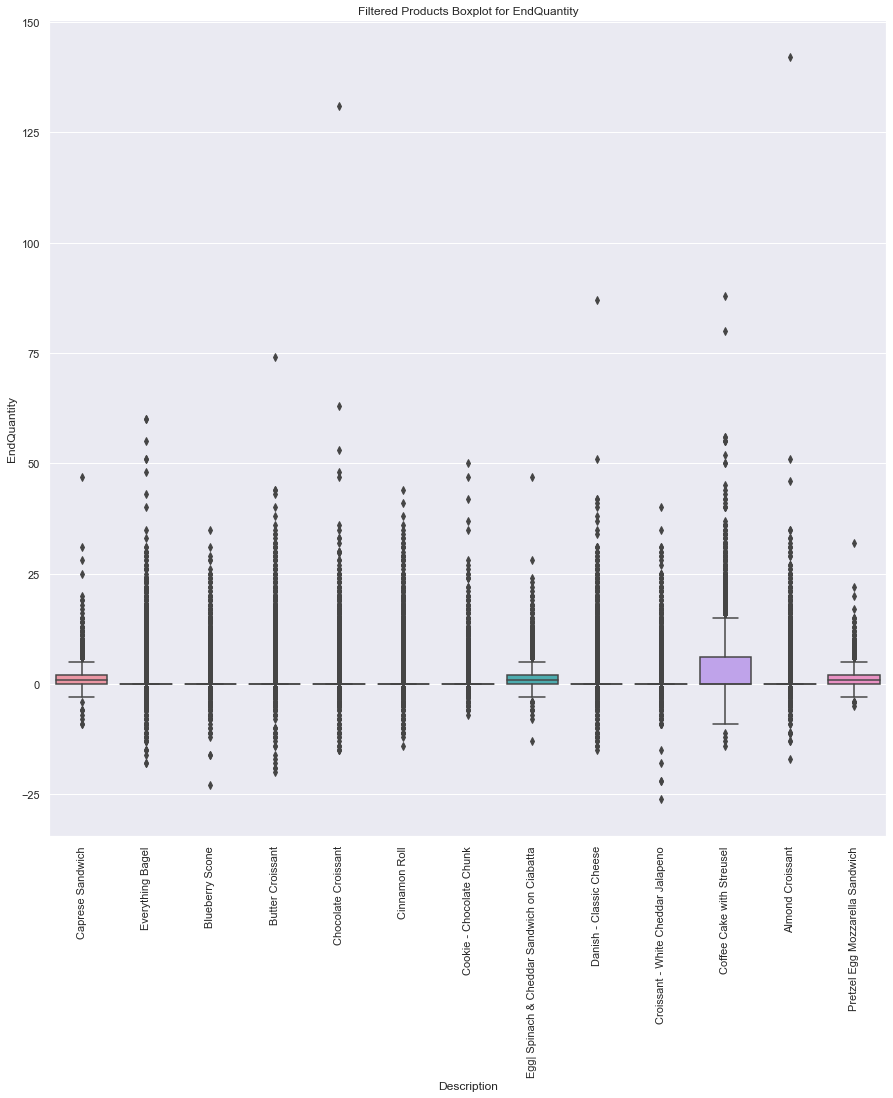
\includegraphics[width = 0.7\linewidth]{figures/figure3.png}
    \caption{Analysis for highest average received quantities }
\end{figure}

For missed sales, we can infer which products may prove to have a slightly higher demand than expected. For products with little or no visible average, we may infer that stores are meeting the demand of customers, perhaps noting a more or less stable inventory of said products. For other products however, having high or often missed sales may mean a re-evaluation on the stocking patterns of these products, as perhaps these products in their current ordering quantities may not be meeting certain demand. 
\begin{figure}[ht]
    \centering
    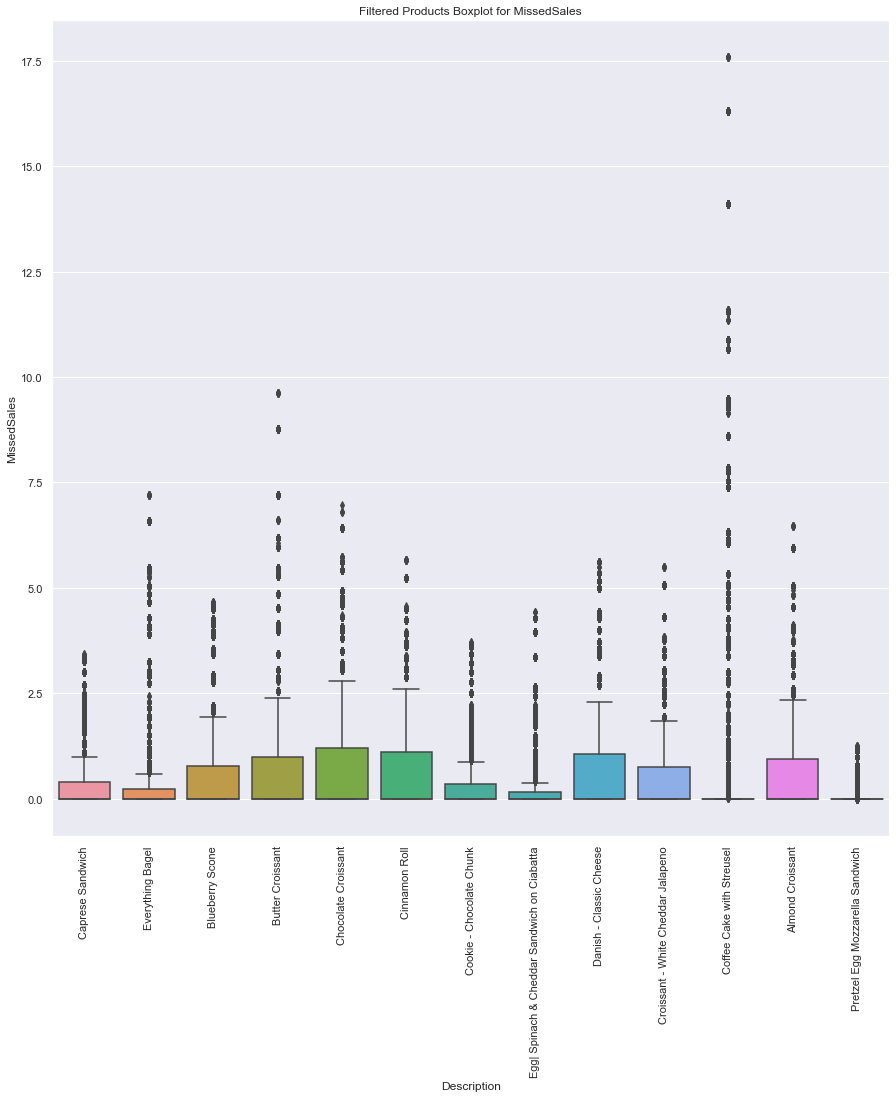
\includegraphics[width = 0.7\linewidth]{figures/figure4.png}
    \caption{Analysis for highest average received quantities }
\end{figure}

\newpage

\subsection{Top 25\% of the product }
We try to further understand the sales trends of the top 25\% of products by visualizing a breakdown of how often these products are received in stores and determine if any pattern or trend can be understood. In this example, we see that for the top 25\% of products there are two patterns, either the amount of products received is very consistent as we see with the coffee cake and everything bagel, or there is a small variance in the amount of product received. It is also worth noting that these product’s received count lie in the range around 5 to 13, true for the top 3 products. 

\begin{figure}[ht]
    \centering
    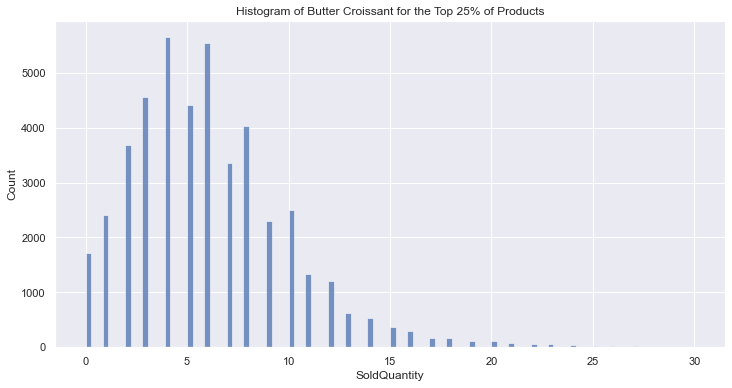
\includegraphics[width = 0.56\linewidth]{figures/figure9.png}
    \caption{Histogram of Butter Croissant }
\end{figure}

\begin{figure}[ht]
    \centering
    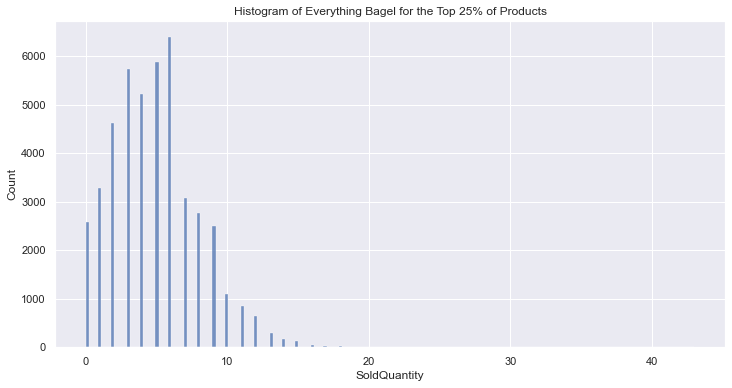
\includegraphics[width = 0.56\linewidth]{figures/figure10.png}
    \caption{Histogram of Bagel }
\end{figure}

\begin{figure}[ht]
    \centering
    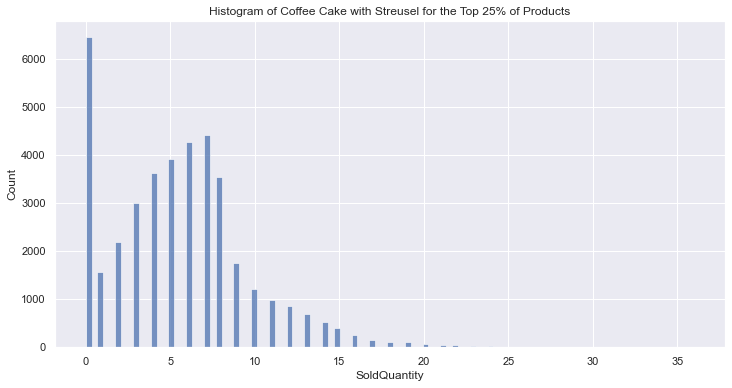
\includegraphics[width = 0.56\linewidth]{figures/figure11.png}
    \caption{Histogram of Coffee Cake }
\end{figure}

Continuing on we look at the sold quantities of these products, and immediately notice a consistent bell curve among all three products peaking between 5 and 8. Here we also want to establish a factor which determines if the products are doing well, and in our opinion we believe that a graph which surpasses half of the count at zero is a good indicator of product performance. When comparing these graphs, what sticks out greatly is the X axis at zero for the coffee cake with streusel graph, as it peaks much higher than the curve’s peak. This may bear investigation later.

The last chart worth looking at is the end quantity of these products, and in our investigation we notice a very great trend towards having zero end quantity per product. Of course, there will be minor outliers which tell us that some products were left over, and out of the top 25\% of products it appears that the coffee cake with streusel does tend to have the most leftover products. However, we do investigate this further into the report.


\subsection{Bottom 25\% of the product }

Continuing on with our investigation, we inspected the bottom 25\% of products to view their patterns, and we immediately noticed how much lower the received quantities for these products are compared to the top 25\%. Here we see a trend skewing slightly closer to zero, indicating perhaps a lower demand or need of these products across all stores

\begin{figure}[ht]
    \centering
    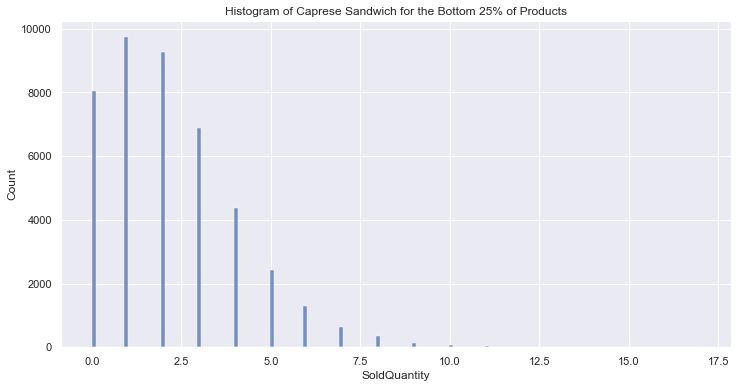
\includegraphics[width = 0.56\linewidth]{figures/figure20.png}
    \caption{Histogram of Caprese }
\end{figure}

\begin{figure}[ht]
    \centering
    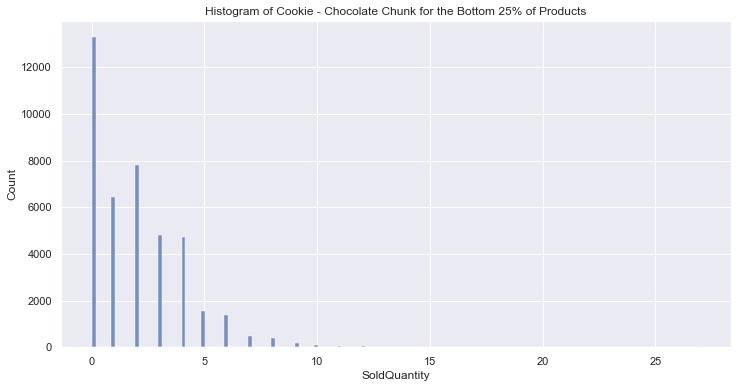
\includegraphics[width = 0.56\linewidth]{figures/figure21.png}
    \caption{Histogram of Cookie }
\end{figure}

\begin{figure}[ht]
    \centering
    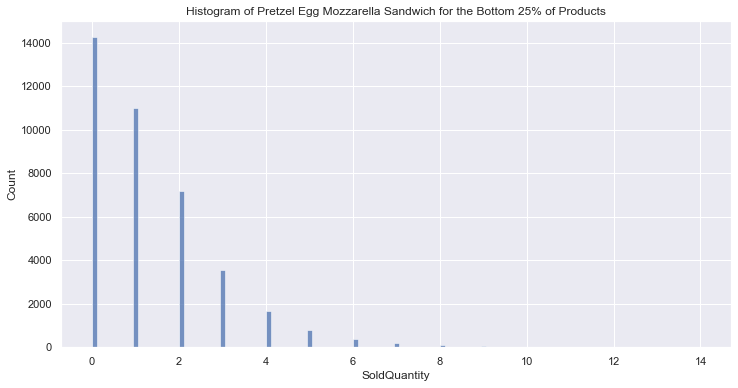
\includegraphics[width = 0.56\linewidth]{figures/figure22.png}
    \caption{Histogram of Mozzarella }
\end{figure}

Of course, considering these to be the bottom 25\% of products, we notice just how much lower they tend to sell. Compared to the top 25\% of products, these products tend to linearly sell much less and present very little or no curve to follow. For example the pretzel egg sandwich and the chocolate cookie commonly does not sell as a product, which should give off red flags and demand evaluation in stocking quantities. 

Lastly, we want to carefully examine the end quantities of these products and see if these products produce more waste. For context, we want the highest peak to be at zero, with all other values to be very very low. Unfortunately, both the pretzel egg and caprese sandwich tend to produce a lot of waste, resulting in tossing of these items and loss of sales.

\subsection{Analysis}

For all stores except 17, 118, and 332 we can compare differences between the top 25\% and bottom 25\% of products based on sales and  understand the differences in stocking, selling, receiving, and how often the products are sold out in general. For each product in top 25\%, each  store will sell, in average, \$16.50 worth of product and retain approximately \$4.80 worth of product by the end of each day. In comparison, the  bottom 25\% of products only sell in average \$8.10 worth of product and retain \$3 by the end of each day. This comes into play when we note that  the stores order around \$35.40 worth of product for the top 25\% of products while stores order \$28.44 worth of product for the bottom 25\% of  product. With this we understand that there exist an unnecessary expense of \$17.44 when purchasing products from the bottom 25\% category  compared to an expense cost of \$14.10. 
We can further break this down by creating a line graph of each product to make inventory trends much more apparent. We first apply this to the  top 25\% of products.

\begin{itemize}
    \item Here we see that in June 2020 the end quantity for the product was very high as compared to sold quantity. 
    \item For the product Everything Bagel in the month of Jan 2020 The quantity received was very high and thus the end quantity was high where as the  sales was less.
\end{itemize}

As we can see, products in the top 25\% category show healthier inventory trends compared to the bottom 25\% category. Products in the top 25\%  category tend to place lower orders than the products received, retaining less product stock and resulting in the items being out of stock more  often as noted by the end quantity. However for products in the bottom 25\% category we see order amounts outweigh the amount receive,  resulting in higher retention of products and leading to higher end quantities in these products. This may demonstrate an unnecessary amount of  overstocking in the bottom 25\% of products, requiring certain re-evaluation when choosing to re-order these items.

Lastly, we must estimate the amount of sales loss per event when product is unavailable. To achieve this, we scan through the data for entries  which state the product is out of stock. If so, we note down the date and the store ID which ran out of stock of the product. Using the date, we  calculate the dates of the previous four weeks and store those dates in a list. Lastly, we can filter through the data and scan for the previous four  dates alongside the store ID and obtain the SoldQuantity entry for each week. We will use these values to calculate the average amount of  product the given store ID has sold, and make the assumption that for the current date the store has missed out on 75\% of those sales. We go  through the entire data frame one product at a time, summing each of those values and get a rough estimate of how much missed sales each of  those products encountered over the course of one year. 
